\documentclass[12pt, oneside]{article}

\usepackage{amssymb,amsmath,pifont,amsfonts,comment,enumerate,enumitem}
\usepackage{currfile,xstring,hyperref,tabularx,graphicx,wasysym}
\usepackage[labelformat=empty]{caption}
\usepackage[dvipsnames,table]{xcolor}
\usepackage{multicol,multirow,array,listings,tabularx,lastpage,textcomp,booktabs}

% NOTE(joe): This environment is credit @pnpo (https://tex.stackexchange.com/a/218450)
\lstnewenvironment{algorithm}[1][] %defines the algorithm listing environment
{   
    \lstset{ %this is the stype
        mathescape=true,
        frame=tB,
        numbers=left, 
        numberstyle=\tiny,
        basicstyle=\rmfamily\scriptsize, 
        keywordstyle=\color{black}\bfseries,
        keywords={,procedure, div, for, to, input, output, return, datatype, function, in, if, else, foreach, while, begin, end, }
        numbers=left,
        xleftmargin=.04\textwidth,
        #1
    }
}
{}
\lstnewenvironment{java}[1][]
{   
    \lstset{
        language=java,
        mathescape=true,
        frame=tB,
        numbers=left, 
        numberstyle=\tiny,
        basicstyle=\ttfamily\scriptsize, 
        keywordstyle=\color{black}\bfseries,
        keywords={, int, double, for, return, if, else, while, }
        numbers=left,
        xleftmargin=.04\textwidth,
        #1
    }
}
{}

\newcommand\abs[1]{\lvert~#1~\rvert}
\newcommand{\st}{\mid}

\newcommand{\A}[0]{\texttt{A}}
\newcommand{\C}[0]{\texttt{C}}
\newcommand{\G}[0]{\texttt{G}}
\newcommand{\U}[0]{\texttt{U}}

\newcommand{\cmark}{\ding{51}}
\newcommand{\xmark}{\ding{55}}



\begin{document}
\begin{flushright}
\StrBefore{\currfilename}{.}
\end{flushright}

\section*{This week's highlights}
\begin{itemize}
\item Define multiple ways for representing numbers
\item Compute the ranges of numbers that can be represented using a given definition
\item Represent negative integers in multiple ways
\item Perform arithmetic operations on integers using multiple representations
\item Relate algorithms for integer operations to bitwise boolean operations
\item List the truth tables and meanings for conjunction, disjunction, exclusive or.
\item Correctly use XOR and bit shifts
\item Relate boolean operations to applications in combinatorial circuits.
\end{itemize}

\section*{Lecture videos}
Week 2 Day 1
\href{https://www.youtube.com/playlist?list=PLML4QilACLk6cXlocBCPCFS9vn_BZmkFa}{YouTube playlist}

Week 2 Day 2
\href{https://youtube.com/playlist?list=PLML4QilACLk5NUKPvXRmw-9FRh2dCOVEU}{YouTube playlist}

Week 2 Day 3
\href{https://youtube.com/playlist?list=PLML4QilACLk4uSylet-RB8mf4bMueVFgK}{YouTube playlist}

\newpage
\section*{Monday January 11}
{\bf Definition} (Rosen p.\ 246) For $b$ an integer greater than $1$ and $n$ a positive integer, 
the {\bf base $b$ expansion of $n$}  is
\[
(a_{k-1} \cdots a_1 a_0)_b
\]
where $k$ is a positive integer, $a_0, a_1, \ldots, a_{k-1}$ are nonnegative integers less than $b$, $a_{k-1} \neq  0$, and
\[
n =  a_{k-1} b^{k-1} + \cdots + a_1b + a_0
\]

\vfill
Algorithm for converting from base $b_1$ expansion to base $b_2$ expansion:

\vfill

{\bf Definition} For $b$ an integer greater than $1$, $w$ a positive integer, and $n$ a nonnegative integer
$\underline{\phantom{\hspace{1in}}}$, ~
the {\bf base $b$ fixed-width $w$ expansion of $n$}  is
\[
(a_{w-1} \cdots a_1 a_0)_{b,w}
\]
where  $a_0, a_1, \ldots, a_{w-1}$ are nonnegative integers less than $b$ and
\[
n =  a_{w-1} b^{w-1} + \cdots + a_1b + a_0
\]


\begin{center}
\begin{tabular}{|c|c|c|c|c|}
\hline
Decimal &  Binary  & Binary fixed-width $10$& Binary fixed-width $7$ & Binary fixed-width $4$\\
$b=10$ & $b=2$ & $b=2$, $w =  10$& $b=2$, $w =  7$& $b=2$, $w =  4$ \\
\hline 
&&&&  \\
$(20)_{10}$&\phantom{$(10100)_{2}$\qquad\qquad}&&  &\\
&&&&  \\
&&&&  \\
\hline
\end{tabular}
\end{center}


\newpage


{\bf Definition} For $b$ an integer greater than $1$, $w$ a positive integer, $w'$ a positive  integer, and $x$ a real number the {\bf base $b$ fixed-width expansion of $x$ with integer part width $w$  and fractional part width $w'$} is
$(a_{w-1} \cdots a_1 a_0 .  c_{1} \cdots c_{w'})_{b,w,w'}$
where  $a_0, a_1, \ldots, a_{w-1}, c_1, \ldots, c_{w'}$ are nonnegative integers less than $b$ and
$$\underline{\phantom{x \geq a_{w-1} b^{w-1} +  \cdots + a_1 b + a_0 +  c_{1} b^{-1} + \cdots +  c_{w'} b^{-w'}}}$$
and
$$\underline{\phantom{x < a_{w-1} b^{w-1} +  \cdots + a_1 b + a_0 +  c_{1} b^{-1} + \cdots +  (c_{w'} +1) b^{-w'}}}$$

\begin{center}
\begin{tabular}{|c|p{5in}|}
\hline
& \\
$3.75$  in fixed-width binary,& \\
integer part width $2$,&\\
 fractional part width $8$ & \\
& \\
\hline
& \\
$0.1$  in fixed-width binary, & \\
integer part width $2$, &\\
 fractional part width $8$ & \\
& \\
\hline
\end{tabular}
\end{center}

\vfill

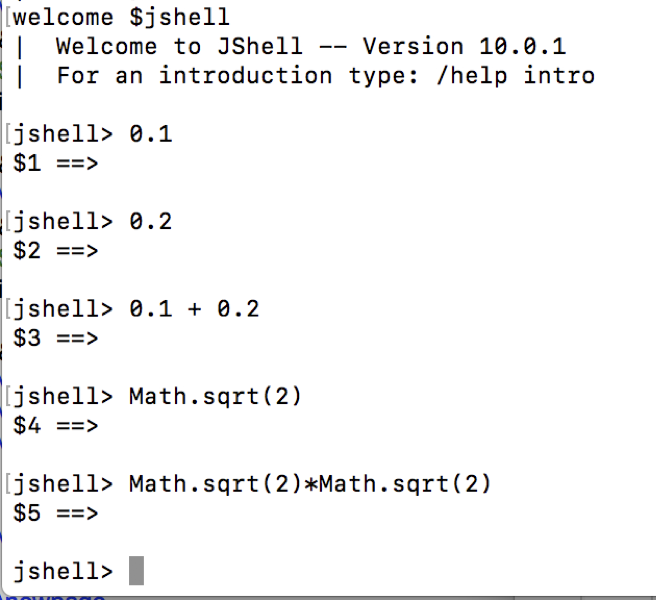
\includegraphics{../Resources/images/ArithmeticDemo.png}

Note: Java uses floating point, not fixed width representation, but similar rounding errors appear in both.
\newpage
\section*{Wednesday January 13}

\begin{center}
\begin{tabular}{|p{3.7in}|p{3.7in}|}
\hline 
&   \\
{\bf base $b$ expansion of $n$}  & {\bf base $b$ fixed-width $w$ expansion of $n$}  \\
& \\
\hline  
For $b$ an integer greater than $1$ and $n$ a positive integer, 
the {\bf base $b$ expansion of $n$}  is $(a_{k-1} \cdots a_1 a_0)_b$
where $k$ is a positive integer, $a_0, a_1, \ldots, a_{k-1}$ are nonnegative integers less than $b$, $a_{k-1} \neq  0$, and $n =  a_{k-1} b^{k-1} + \cdots + a_1b + a_0$
& 
For $b$ an integer greater than $1$, $w$ a positive integer, and $n$ a nonnegative integer
with $n <  b^w$, the {\bf base $b$ fixed-width $w$ expansion of $n$}  is
$(a_{w-1} \cdots a_1 a_0)_{b,w}$
where  $a_0, a_1, \ldots, a_{w-1}$ are nonnegative integers less than $b$ and 
$n =  a_{w-1} b^{w-1} + \cdots + a_1b + a_0$\\
\hline
\end{tabular}
\end{center}
\vfill

{\bf Representing negative integers in binary}: Fix a positive integer  width for the representation  $w$, $w >1$.

\begin{tabular}{|cc|p{3.4in}|p{3.7in}|}
\hline
& & To  represent a positive integer $n$ & To represent a negative integer $-n$\\
\hline
&& &  \\
&\parbox[t]{2mm}{\multirow{4}{*}{\rotatebox[origin=c]{90}{Sign-magnitude}}} &
$[ 0a_{w-2} \cdots a_0]_{s,w}$, where $n =  (a_{w-2} \cdots a_0)_{2,w-1}$& 
$[1a_{w-2} \cdots a_0]_{s,w}$
, where $n =  (a_{w-2} \cdots a_0)_{2,w-1}$\\
&& & \\
&& Example $n=17$, $w=7$:  & Example $-n=-17$, $w=7$: \\
&& & \\
&& & \\
&& & \\
\hline
&&  &  \\
&\parbox[t]{2mm}{\multirow{4}{*}{\rotatebox[origin=c]{90}{2s complement}}} &
$[0a_{w-2} \cdots a_0]_{2c,w}$, where $n =  (a_{w-2} \cdots a_0)_{2,w-1}$& $[1a_{w-2} \cdots a_0]_{2c,w}$, where $2^{w-1} - n =  (a_{w-2} \cdots a_0)_{2,w-1}$\\
&& & \\
&& Example $n=17$, $w=7$:  & Example $-n=-17$, $w=7$: \\
&& & \\
&& & \\
&& & \\
\hline
&&  &  \\
\parbox[t]{1.5mm}{\multirow{4}{*}{\rotatebox[origin=c]{90}{{\it Extra example:}}}} 
& \parbox[t]{2mm}{\multirow{4}{*}{\rotatebox[origin=c]{90}{1s complement}}} &
$[0a_{w-2} \cdots a_0]_{1c,w}$, where $n =  (a_{w-2} \cdots a_0)_{2,w-1}$& $[1\bar{a}_{w-2} \cdots \bar{a}_0]_{1c,w}$, where $n =  (a_{w-2} \cdots a_0)_{2,w-1}$ and we define  $\bar{0} = 1$ and $\bar{1} = 0$.\\
&& & \\
&& Example $n=17$, $w=7$:  & Example $-n=-17$, $w=7$: \\
&& & \\
&& & \\
&& & \\
\hline
\end{tabular}
\vfill

{\bf Representing $0$}:

\vfill
\newpage
{\bf Fixed-width addition}: adding one bit at time, using the usual column-by-column and carry arithmetic, and dropping the carry from the leftmost column so the result is the same width as the summands.  {\it Does this give the right value for the sum?}
\begin{multicols}{3}
\begin{align*}
   & (1~ 1~ 0~ 1~ 0~ 0)_{2,6}\\
+ & (0~ 0~ 0~ 1~ 0~ 1)_{2,6}\\
&\overline{\phantom{(1~1~1~0~0~1)_{2,6}}}\\
\end{align*}

\begin{align*}
   & [1~ 1~ 0~ 1~ 0~ 0]_{s,6}\\
+ & [0~ 0~ 0~ 1~ 0~ 1]_{s,6}\\
&\overline{\phantom{(1~1~1~0~0~1)_2}}\\
\end{align*}

\begin{align*}
   & [1~ 1~ 0~ 1~ 0~ 0]_{2c,6}\\
+ & [0~ 0~ 0~ 1~ 0~ 1]_{2c,6}\\
&\overline{\phantom{(1~1~1~0~0~1)_2}}\\
\end{align*}
\end{multicols}

\vfill
{\it Extra example}

\vspace{-25pt}

\begin{multicols}{3}
\begin{align*}
   & (1~ 1~ 0~ 1~ 0~ 0)_{2,6}\\
\times & (0~ 0~ 0~ 1~ 0~ 1)_{2,6}\\
&\overline{\phantom{(1~1~1~0~0~1)_{2,6}}}\\
\end{align*}

\begin{align*}
   & [1~ 1~ 0~ 1~ 0~ 0]_{s,6}\\
\times & [0~ 0~ 0~ 1~ 0~ 1]_{s,6}\\
&\overline{\phantom{(1~1~1~0~0~1)_2}}\\
\end{align*}

\begin{align*}
   & [1~ 1~ 0~ 1~ 0~ 0]_{2c,6}\\
\times & [0~ 0~ 0~ 1~ 0~ 1]_{2c,6}\\
&\overline{\phantom{(1~1~1~0~0~1)_2}}\\
\end{align*}
\end{multicols}


\vfill

\newpage
\section*{Friday January 15}
\begin{center}
\begin{tabular}{p{2in}p{2in}p{2in}}
\begin{center}\begin{tabular}{cc|c}
\multicolumn{2}{c|}{Input}  & Output \\
$x$ & $y$ & $x \text{ AND } y$  \\
\hline
$1$ & $1$ & $1$\\
$1$ & $0$ & $0$\\
$0$ & $1$ & $0$\\
$0$ & $0$ & $0$\\
\end{tabular}\end{center}
&
\begin{center}\begin{tabular}{cc|c}
\multicolumn{2}{c|}{Input}  & Output \\
$x$ & $y$ & $x \text{ XOR } y$  \\
\hline
$1$ & $1$ & $0$\\
$1$ & $0$ & $1$\\
$0$ & $1$ & $1$\\
$0$ & $0$ & $0$\\
\end{tabular}\end{center}
&
\begin{center}\begin{tabular}{c|c}
Input  & Output \\
$x$ & $\text{NOT } x$  \\
\hline
$1$ & $0$\\
$0$ & $1$\\
\end{tabular}\end{center}\\
\begin{center}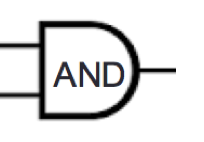
\includegraphics[height=0.6in]{../Resources/images/xANDy.png}\end{center}
& \begin{center}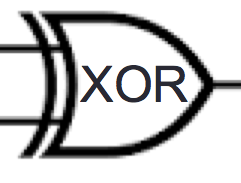
\includegraphics[height=0.4in]{../Resources/images/xXORy.png} \end{center}
&\begin{center}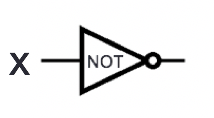
\includegraphics[height=0.5in]{../Resources/images/NOTx.png} \end{center}
\end{tabular}
\end{center}

\vspace{-40pt}

{\bf Example digital circuit}: 

\begin{multicols}{2}
\begin{center}
   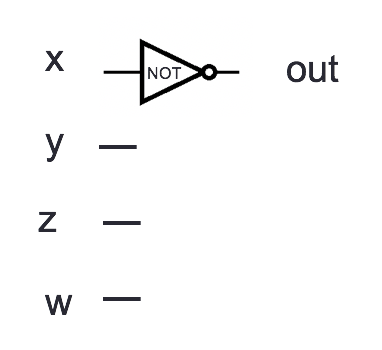
\includegraphics[width=1.2in]{../Resources/images/circuitEx.png} 
\end{center}
\columnbreak
Output when $x=1, y=0, z=0, w = 1$ is \underline{\phantom{$~~~0~~~$}}
Output when $x=1, y=1, z=1, w = 1$ is \underline{\phantom{$~~~0~~~$}}
Output when $x=0, y=0, z=0, w = 1$ is \underline{\phantom{$~~~0~~~$}}
\phantom{Output when $x=0, y=0, z=0, w = 0$ is \underline{\phantom{$~~~0~~~$}}}
\end{multicols}



Draw a logic circuit with inputs $x$ and $y$ whose output  is always $0$.  {\it  Can you use exactly 1 gate?}


\vspace{40pt}

{\bf Fixed-width addition}: adding one bit at time, using the usual column-by-column and carry arithmetic, and dropping the carry from the leftmost column so the result is the same width as the summands.  In many cases, this gives representation of the correct value for the sum when we interpret the summands
in fixed-width binary or in 2s complement.

For single column:
\begin{center}
\begin{tabular}{cc|cc}
\multicolumn{2}{c|}{Input}  & \multicolumn{2}{|c}{Output}  \\
$x_0$ & $y_0$ & $s_0$ & $c_0$  \\
\hline
$1$ & $1$ & \phantom{$0$} & \phantom{$1$} \\
$1$ & $0$ & \phantom{$1$} & \phantom{$0$}\\
$0$ & $1$ & \phantom{$1$} & \phantom{$0$}\\
$0$ & $0$ & \phantom{$0$} & \phantom{$0$}\\
\end{tabular}
\end{center}

\begin{center}
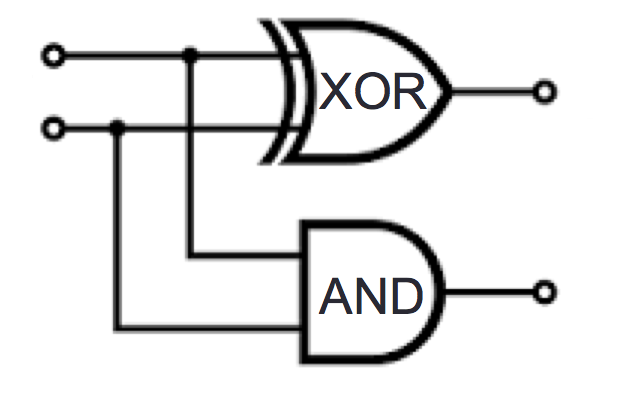
\includegraphics[width=1.5in]{../Resources/images/half-adder.png}x
\end{center}

\newpage
Draw a logic circuit that implements fixed-width 2 binary addition:
\begin{itemize}
\item Inputs  $x_0, y_0, x_1, y_1$ represent $(x_1  x_0)_{2,2}$ and $(y_1 y_0)_{2,2}$
\item Outputs  $z_0, z_1, z_2$ represent $(z_2  z_1 z_0)_{2,3} = (x_1  x_0)_{2,2} + (y_1 y_0)_{2,2}$ (may require up to width  $3$)
\end{itemize}

{\it First approach}: half-adder for each column, then combine carry from right column with sum of left column

\vfill



Write expressions for the circuit output values in terms of input values:

%\vspace{-10pt}

$z_0 = \underline{\phantom{x_0 \oplus y_0\hspace{3in}}}$

%\vspace{-10pt}

$z_1 = \underline{\phantom{(x_1 \oplus y_1) \oplus c_0}\hspace{2.5in}}$ \phantom{where $c_0 = x_0 \land y_0$}

%\vspace{-10pt}

$z_2 = \underline{\phantom{(c_0 \land (x_1 \oplus y_1)) \oplus c_1}\hspace{2in}}$ \phantom{where $c_1 = x_1 \land y_1$}\\

{\it Second approach}: for middle column, first add carry from right column to $x_1$, then add result to $y_1$

\vfill


Write expressions for the circuit output values in terms of input values:

%\vspace{-10pt}

$z_0 = \underline{\phantom{x_0 \oplus y_0}\hspace{3in}}$

%\vspace{-10pt}

$z_1 = \underline{ \phantom{(c_0 \oplus x_1) \oplus y_1}\hspace{2.4in}}$ \phantom{where $c_0 = x_0 \land y_0$}

%\vspace{-10pt}

$z_2 = \underline{\phantom{(c_0 \land x_1) \oplus ((c_0 \oplus x_1)\land y_1)}\hspace{1.5in}}$\\

{\it Extra example} Describe how to generalize this addition circuit for larger width inputs.


\section*{Review quiz questions}
\begin{enumerate}

\item Recall the definitions from class for number representations for {\bf base $b$ expansion of $n$},
{\bf  base $b$ fixed-width $w$ expansion of $n$}, and {\bf base $b$ fixed-width expansion of $x$ 
with integer part width $w$ and fractional part width $w'$}.

For example, the base $2$ (binary) expansion of $4$ is 
$\qquad
(100)_2 \qquad$
and the base $2$ (binary) fixed-width $8$ expansion of $4$ is
$\qquad
(00000100)_{2,8} \qquad$
and the base $2$ (binary) fixed-width expansion of $4$ with integer part width $3$ and fractional
part width $2$ of $4$ is
$\qquad
(100.00)_{2,3,2} \qquad$

Compute the listed expansions.  Enter your number using the notation for base 
expansions with parentheses but without subscripts. For example, 
if your answer were $(100)_{2,3}$
you would type \texttt{(100)2,3} into Gradescope.

\begin{enumerate}
\item Give the binary (base $2$) expansion of the number whose octal (base $8$) expansion is
\[
(371)_8
\]
\item Give the decimal (base $10$) expansion of the number whose octal (base $8$) expansion is
\[
(371)_8
\]
\item Give the octal (base $8$) fixed-width $3$ expansion of $(9)_{10}$?
\item Give the ternary (base $3$) fixed-width $8$ expansion of $(9)_{10}$?
\item Give the hexadecimal (base $16$) fixed-width $6$ expansion of
$(16711935)_{10}$?\footnote{This matches a frequent debugging task --
sometimes a program will show a number formatted as a base $10$
integer that is much better understood with another representation.}
\item Give the hexadecimal (base $16$) fixed-width $4$ expansion of
$$(1011~ 1010 ~ 1001~ 0000 )_2$$
Note: the spaces between each group of 4 bits above are for your convenience only.  How
might they help your calculations?
\item Give the binary fixed width expansion of $0.125$ with integer part width $2$ and 
fractional part width $4$.
\item Give the binary fixed width expansion of $0.1$ with integer part width $2$ and 
fractional part width $3$.
\end{enumerate}

\item Select all and only the correct choices below.
\begin{enumerate}
\item Suppose you were told that the positive integer $n_1$ has the property that $n_1 \textbf{ div } 2 = 0$. Which of the following can you conclude?
\begin{enumerate}
\item $n_1$ has a binary (base $2$) expansion
\item $n_1$ has a ternary (base $3$) expansion
\item $n_1$ has a hexadecimal (base $16$) expansion
\item $n_1$ has a base $2$ fixed-width $1$ expansion
\item $n_1$ has a base $2$ fixed-width $20$ expansion
\end{enumerate}
\item Suppose you were told that the positive integer $n_2$ has the property that $n_2 \textbf{ mod } 4 = 0$. Which of the following can you conclude?
\begin{enumerate}
\item the leftmost symbol in the binary (base $2$) expansion of $n_2$ is $1$
\item the leftmost symbol in the base $4$ expansion of $n_2$ is $1$
\item the rightmost symbol in the base $4$ expansion of $n_2$ is $0$
\item the rightmost symbol in the octal (base $8$) expansion of $n_2$ is $0$
\end{enumerate}
\end{enumerate}
\item Recall the definitions of signed integer representations from class: sign-magnitude and 2s complement.

\begin{enumerate}
    \item Give the 2s complement width 6 representation of the number represented in binary fixed-width 6
    representation as $(001011)_{2,6}$. 
    \item Give the 2s complement width 4 representation of the number represented in sign-magnitude
    width 4 as $[1111]_{s,4}$.
    \item Give the sign magnitude width 4 representation of the number represented in 2s complement
    width 4 as $[1111]_{2c,4}$.
    \item In binary fixed-width addition (adding one bit at time, using the usual column-by-column and carry arithmetic, and ignoring the carry from the  leftmost column), we get: 
    \begin{align*}
        &1110  \qquad  \text{first summand}\\
        +&0100 \qquad  \text{second summand}\\
        &\overline{0010} \qquad \text{result}
    \end{align*}
    Select all and only the  true  statements below:
    \begin{enumerate}
        \item When interpreting each of the summands and the result in binary fixed-width 4, 
        the result represents the actual value of the sum of the summands.
        \item When interpreting each of the summands and the sum in sign-magnitude width 4, the result  
        represents the actual value of the sum of the summands.
        \item When interpreting each of the summands and the sum in 2s complement width 4, the result 
        represents the actual value of the sum of the summands.
    \end{enumerate}    
    \item In binary fixed-width addition (adding one bit at time, using the usual column-by-column and carry arithmetic, and ignoring the carry from the  leftmost column), we get: 
    \begin{align*}
        &0110  \qquad  \text{first summand}\\
        +&0111 \qquad  \text{second summand}\\
        &\overline{1101} \qquad \text{result}
    \end{align*}
    Select all and only the  true  statements below:
    \begin{enumerate}
        \item When interpreting each of the summands and the result in binary fixed-width 4, 
        the result represents the actual value of the sum of the summands.
        \item When interpreting each of the summands and the sum in sign-magnitude width 4, the result  
        represents the actual value of the sum of the summands.
        \item When interpreting each of the summands and the sum in 2s complement width 4, the result 
        represents the actual value of the sum of the summands.
    \end{enumerate}   
\end{enumerate}

\item 
\begin{enumerate}
\item Consider the logic circuit
    \begin{center}
    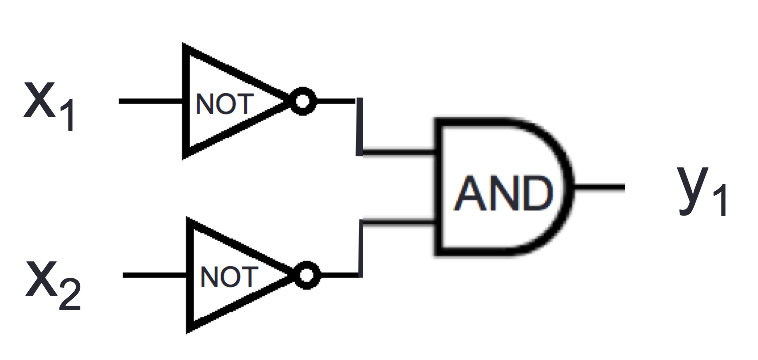
\includegraphics[width=2in]{../Resources/images/review-circuit-1.png}
    \end{center}
    Calculate the value of the output of this circuit ($y_1$) for each of the following settings(s) of input values.
    \begin{enumerate}
        \item $x_1 = 1$, $x_2 = 1$
        \item $x_1 = 1$, $x_2 = 0$
        \item $x_1 = 0$, $x_2 = 1$
        \item $x_1 = 0$, $x_2 = 0$
    \end{enumerate}  \item Consider the logic circuit
    \begin{center}
    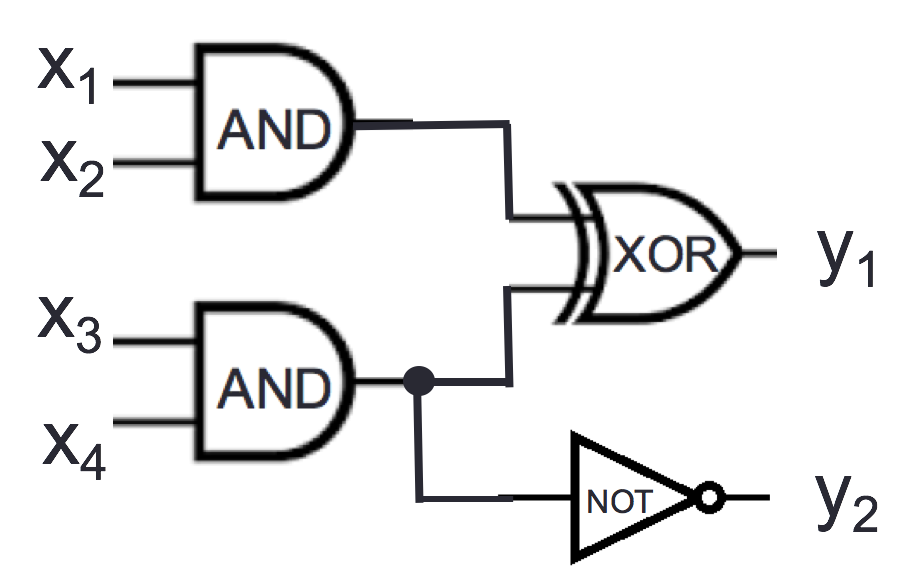
\includegraphics[width=2in]{../Resources/images/review-circuit-2.png}
    \end{center}
    For which of the following settings(s) of input values is the output
    $y_1 = 0$, $y_2 = 1$. (Select all and only those that apply.)
    \begin{enumerate}
        \item $x_1 = 0$, $x_2 = 0$, $x_3 = 0$, and $x_4 = 0$
        \item $x_1 = 1$, $x_2 = 1$, $x_3 = 1$, and $x_4 = 1$
        \item $x_1 = 1$, $x_2 = 0$, $x_3 = 0$, and $x_4 = 1$
        \item $x_1 = 0$, $x_2 = 0$, $x_3 = 1$, and $x_4 = 1$
    \end{enumerate}
  
\end{enumerate}


\end{enumerate}
\end{document}
